%%%%%%%%%%%%%%%%%%%%%%%%%%%%%%%%%%%%%%%%%%%%%%%%%%%%%%%%%%%%%%%%%%%%%%%%%%%%%%%%
%2345678901234567890123456789012345678901234567890123456789012345678901234567890
%        1         2         3         4         5         6         7         8

\documentclass[letterpaper, 10 pt, conference]{ieeeconf}  % Comment this line out
                                                          % if you need a4paper
%\documentclass[a4paper, 10pt, conference]{ieeeconf}      % Use this line for a4
                                                          % paper

\IEEEoverridecommandlockouts                              % This command is only
                                                          % needed if you want to
                                                          % use the \thanks command
\overrideIEEEmargins

\usepackage{times}
\usepackage[T1]{fontenc}
\usepackage{tikz}
\usepackage{amsmath}
%\usepackage{amsthm}
%\usepackage{verbatim}
\usepackage{subfigure}
\usepackage{graphicx}
\usepackage{wrapfig}

\newcommand{\comments}[1]{}
% See the \addtolength command later in the file to balance the column lengths
% on the last page of the document



% The following packages can be found on http:\\www.ctan.org
\usepackage{graphics} % for pdf, bitmapped graphics files
\usepackage{epsfig} % for postscript graphics files
\usepackage{mathptmx} % assumes new font selection scheme installed
\usepackage{times} % assumes new font selection scheme installed
\usepackage{amsmath} % assumes amsmath package installed
\usepackage{amssymb}  % assumes amsmath package installed

\usepackage{amsmath}
\interdisplaylinepenalty=2500

\title{\LARGE \bf
The Conjugate Unscented Transform- CUT
}
\comments{
\author{ \parbox{3 in}{\centering Huibert Kwakernaak*
         \thanks{*Use the $\backslash$thanks command to put information here}\\
         Faculty of Electrical Engineering, Mathematics and Computer Science\\
         University of Twente\\
         7500 AE Enschede, The Netherlands\\
         {\tt\small h.kwakernaak@autsubmit.com}}
         \hspace*{ 0.5 in}
         \parbox{3 in}{ \centering Pradeep Misra**
         \thanks{**The footnote marks may be inserted manually}\\
        Department of Electrical Engineering \\
         Wright State University\\
         Dayton, OH 45435, USA\\
         {\tt\small pmisra@cs.wright.edu}}
}
}
\author{\begin{tabular}{cccc}
 Nagavenkat Adurthi  &  Puneet Singla &  Tarunraj Singh \\
Graduate Student & Assistant Professor & Professor \\
nagavenk@buffalo.edu & psingla@buffalo.edu & tsingh@buffalo.edu \vspace{0.01in}\end{tabular}\\
%\textsl{Department of Mechanical \& Aerospace Engineering}\\
\textsl{University at Buffalo, State University of New York,
Amherst, NY 14260-4400}}

\begin{document}



\maketitle
\thispagestyle{empty}
\pagestyle{empty}


%%%%%%%%%%%%%%%%%%%%%%%%%%%%%%%%%%%%%%%%%%%%%%%%%%%%%%%%%%%%%%%%%%%%%%%%%%%%%%%%
\begin{abstract}
This paper presents methods to evaluate fully symmetric sigma points with positive weights for the Unscented Transform that can capture higher order moments of the normal probability density function. This work can be considered as a potenstial extension to the $2n+1$ Unscented Transform rule for nonlinear filtering or it can be used as an efficient Gaussian Cubature rule with reduced number of points compared to the Gauss Hermite product rule. Mainly three sets of sigma points are explored, firstly the set of sigma points of 'CUT4' that are 4th degree exact for any dimension. Secondly, the set of sigma points of 'CUT6' that are 6th degree exact for dimensions $2 \le N \le 9 $ and thirdly the set of sigma points of CUT8 that are 8th degree exact for dimensions $2 \le N \le 6 $ . Each method is compared to the Gauss Hermite product rule which is known to be exact for polynomial functions. The results are very encouraging for the fact that the same order of accuracy can be achieved with the a small fraction of the number of points used by the Gauss Hermite product rule. Finally results for a few non-polynomial type functions are shown that would motivate the idea to develop even higher order set of sigma points with reduced number of points.             
\end{abstract}


%%%%%%%%%%%%%%%%%%%%%%%%%%%%%%%%%%%%%%%%%%%%%%%%%%%%%%%%%%%%%%%%%%%%%%%%%%%%%%%%
\section{INTRODUCTION}

\indent\indent Integrals involving the normal probability density function such as in (\ref{exptint}) frequently arise in statistics and filtering and often do not have an analytical answer. One would have to resort to numerical computation methods such as the Gauss Hermite quadrature rule, where the quadrature points are the roots of Hermite polynomial of required degree. For 1 dimensional integrals the Gauss Hermite quadrature rules are simple to compute or are well documented, are accurate and are by far the minimal number of points required. To evaluate higher dimensional integrals, the quadrature points(now called cubature for $N\ge2$) can be constructed from the 1 dimensional quadrature points, which gives rise to the 'Gauss Hermite Product rule'. A complete description on product rules can be found in chapter 3 of \cite{c1}. In 1 dimensional integrals, 'm' quadrature points are required for a polynomial of degree $2m-1$, the proof of which is given in \cite{c1}. Hence for a N-dimensional system one would require $m^N$ cubature points. This number grows exponentially with the dimension. Even for a lower dimension such as 6, the number of points required to evaluate the integral when $f(x)$ is a polynomial of degree 9 is $5^6=15625$. This is a huge number of points that might be computationally expensive to use especially when the evaluation of $f(x)$ at each cubature point is in itself expensive. But fortunately the Gauss Hermite product rule is \emph{not minimal},with reference to \cite{c1}, and there exists cubature rules with reduced number of points. This forms the basis of our motivation to develop efficient cubature methods.\newline
 \indent\indent An extensive amount of work has been done in this field to develop cubature rules with fewer points. Particularly \cite{c2} where the author has developed non-product gaussian cubature rules for second, third and fifth degree polynomials in any dimension. In general to develop a cubature rule that is applicable to any dimension is a difficult procedure. Thus the main focus has been to construct cubature rules only for few lower dimension integrals but to a higher degree with minimal number of points. A cubature rule of degree 2 with $N+1$ points and a cubature method of degree 3 with $2N$ points is developed in \cite{c3} for a general centrally symmetric weight function such as the normal and uniform PDF and it is claimed that this is the minimum number of points possible. In \cite{c4} a fully symmetric integration rules with minimal points for 2-Dimension are developed that are exact for degree 9-15.  A 19 point cubature rule is developed in \cite{c5} for symmetric regions in 2-dimensions that are exact for degree 9. For a 2D integral, with symmetric weight function such as normal or unifrom, a 12 point cubature rule for degre 7  is developed in \cite{c6}. It is even claimed that this is the minimal number of points required and there exist many such 12 point cubature rule for degree 7 in 2D system.\newline
  \indent\indent Most of the non-product cubature rule possess certain similarities, they exploit the symmetry of the weight function, assume a structure for the cubature points, solve a system of nonlinear equations. Hence these methods also suffer some similar drawbacks such as inconsistency of the set of nonlinear equations, the presence of negative weights and inability to provide a generalised solution that works for any dimension. The present work heads in the similar manner and tries to overcome some of these difficulties. Thus the primary objective of this paper can be stated as "'To find a sigma point set with reduced number of points that is \emph{equivalent} to the set of quadrature points of Gauss-Hermite Product rule of \emph{same order}. By \emph{equivalent to same order} we mean that for a polynomial of order $2m-1$, both the new reduced sigma point set from the Conjugate Unscented Transform method and the $m^N$ quadrature points from Gauss-Hemrite product rule result in same order of relative error compared to the 'true value'.


\subsection{Importance of Higher-Order Moments}
Consider the integral in (\ref{exptint}) for evaluating the true expected value of a function and also the approximated expected value in (\ref{exptinttaylor}) using Taylor series expansion of the function about the mean of the Gaussian PDF.
\setlength{\arraycolsep}{0.0em}
\begin{eqnarray}
E[f(x)]&{}={}& \int{f(x)N(x,\mu|P)}dx \label{exptint}\\
E[f(x)]&{}={}& f(\mu)+\nabla{f(\mu)}E[\delta{x}]+\frac{1}{2!}\nabla^2f(\mu)E[\delta{x}^2]\nonumber \\ 
&&{+}\: \frac{1}{3!}\nabla^3f(\mu)E[\delta{x}^3]+\frac{1}{4!}\nabla^4f(\mu)E[\delta{x}^4]... \label{exptinttaylor}
\end{eqnarray}
\setlength{\arraycolsep}{5pt}
where $\delta{x}=(x-\mu)$. To elaborate, when more sigma points are evaluated such that they can satisfy the higher order moment constraint equations (\ref{momentconst}), the integral value evaluated by (\ref{sigmasum}) tends to converge to the 'true' value of the integral. By 'true' value we mean the analytical answer if it is available or the \emph{converged} numerical value evaluated by the Gauss-Hermite product rule. The word \emph{converged} is stressed because for a non-polynomial function one usually does not know the adequate number of points for convergence.More the  higher order moments are captured more is the integral value closer to the 'true value'.

\subsection{Sigma Point Set to capture moments of Gaussian PDF}
With out loss of generality consider a Gaussian PDF with $0$ mean and identity covariance of appropriate dimension. Under this assumption all the odd order central and raw moments of the Gaussian PDF are 0. For a sigma point set $x_1,x_2,...,x_n$ with corresponding weights $w_1,w_2,...w_3$, the expected value or weighted integral value is approximated by a weighted sum as in (\ref{sigmasum}). Consider the Taylor series approximation of the function value at each point about the mean as in (\ref{sigmataylor}) which are then substituted in (\ref{sigmasum}). The resultant equation is in terms of the sigma points and weight chosen. Upon comparing the coefficients of (\ref{compeqnssigtotay}) to (\ref{exptinttaylor}), the resulting set of equations are called the moment constraint eqautions (\ref{momentconst}).   
\setlength{\arraycolsep}{0.0em}
\begin{eqnarray}
E[f(x)]&{}={}& \sum_{i=1}^n{w_if(x_i)}\label{sigmasum}\\
f(x_i)&{}={}& f(0)+\frac{1}{2!}\nabla^2f(0)x_i^2\nonumber \\ 
&&{+}\: \frac{1}{4!}\nabla^4f(0)x_i^4+\frac{1}{6!}\nabla^6f(0)x_i^6... \label{sigmataylor}\\
E[f(x)]&{}={}& f(0)(\sum_{i=1}^n{w_i})+\frac{1}{2!}\nabla^2f(0)(\sum_{i=1}^n{w_ix_i^2})\nonumber\\
&&{+}\: \frac{1}{4!}\nabla^4f(0)(\sum_{i=1}^n{w_ix_i^4})+\frac{1}{6!}\nabla^6f(0)(\sum_{i=1}^n{w_ix_i^6}) \label{compeqnssigtotay}
\end{eqnarray}
\setlength{\arraycolsep}{5pt} 
\setlength{\arraycolsep}{0.0em}
\begin{eqnarray}
\sum_{i=1}^n{w_i}=1, \quad  \sum_{i=1}^n{w_ix_i^2}=E[\delta{x}^2], \quad \sum_{i=1}^n{w_ix_i^4}=E[\delta{x}^4], \nonumber\\
\sum_{i=1}^n{w_ix_i^6}=E[\delta{x}^6]\quad,..., \quad \sum_{i=1}^n{w_ix_i^m}=E[\delta{x}^m]\label{momentconst}
\end{eqnarray}
\setlength{\arraycolsep}{5pt}        
%%%%%%%%%%%%%%%%%%%%%%%%%%%%%%%%%%%%%%%%%%%%%%%%%%%%%%%%%%%%%%%%%%%%%%%%%%%%%%%%
%%%%%%%%%%%%%%%%%%%%%%%%%%%%%%%%%%%%%%%

\section{Methodology to solve the moment constraint equations}
A common methodology that is followed throughout the paper can be summarized as
\begin{enumerate}
\item As we know that the Gaussian PDF is symmetric, we exploit this by constraining the sigma points to various axis.  We later define some of these axis as and when they are required.
\item Sigma points on the same axis  are equidistant from the mean and have equal weight. For the $i^{th}$  set of axis , the distance scaling variables are labeled $r_i$ and weight variables are labeled $w_i$.
\item We find all the moments of the continuous multidimensional normal PDF. The moments of a normal PDF are given by the Isserlis theorem which is formally restated in \cite{c7} 
\item We enumerate the list of points and then form the moment constraint equations till required order in terms of the variable $r_i$ and $w_i$. For example the moment constraint equations till order 4 for a 2D system are shown in Table \ref{moment_match}. The $(x_i,y_i)$ points are enumerated in terms of distance $r_i$. 
\item These equations are solved for $r_i$ and $w_i$, that give the sigma point set.
\end{enumerate}
\begin{table}
\caption{Moment Constraint equations for 2D till order 4}
\label{moment_match}
\begin{center}
\begin{tabular}{|c|c||c|c|}
\hline
Continuous & Discrete & Continuous & Dicrete\\
\hline
$E[x]$ & $\sum_{i=1}^n{w_ix_i}$& $E[y]$ & $\sum_{i=1}^n{w_iy_i}$\\
\hline
$E[x^2]$ & $\sum_{i=1}^n{w_ix_i^2}$& $E[xy]$ & $\sum_{i=1}^n{w_ix_iy_i}$\\
\hline
$E[y^2]$ & $\sum_{i=1}^n{w_iy_i^2}$& $E[x^4]$ & $\sum_{i=1}^n{w_ix_i^2}$ \\
\hline
$E[y^4]$ & $\sum_{i=1}^n{w_iy_i^2}$& $E[x^3y]$ & $\sum_{i=1}^n{w_ix_i^3y_i}$\\
\hline
$E[y^3x]$ & $\sum_{i=1}^n{w_iy_i^3x_i}$ & $E[x^2y^2]$ & $\sum_{i=1}^n{w_ix_i^2y_i^2}$\\
\hline
\end{tabular}
\end{center}
\end{table}
%%%%%%%%%%%%%%%%%%%%%%%%%%%%
\subsection{Sigma points that are $2^{nd}$ moment equivalent}
Sigma points that are $2^{nd}$ moment equivalent can completely satisfy the moment constraint equations till $2^{nd}$ order. To facilitate with the analysis in this section the following definition is introduced with respect to a zero mean and identity covariance matrix Normal PDF \newline 
\emph{Principal axis}: The orthogonal axis in cartesian space intersecting at the origin. These are the axis corresponding to each column of the identity covariance matrix. Thus there are $N$ principal axis or $2N$ distinct points on the principal axis for N-Dimensional system.  We list the points on principal axis as 
\setlength{\arraycolsep}{0.0em}
\begin{eqnarray}
\sigma_i &\in \{\pm\sqrt{P}_j|\{j\}\in\{1,2,...,N\}\}\\
i&=1,2,3,...,2N. 
\end{eqnarray}
\setlength{\arraycolsep}{5pt} 


%%%%%%%%%%%%%%%%%%%%%%%%%%%%%%%%%%%%%%%%%%%%%%%%%%%%%,%%%%%%%%%%%%%%%%%%%%%%%%

\subsubsection{Sigma points constrained to the principal axis}
For an i.i.d random variables $(X_1,X_2,...,X_N)$ the N-Dimensional normal PDF has Identity covariance and zero mean. The first four moments are
\setlength{\arraycolsep}{0.0em}
\begin{eqnarray}
E[X_i^2]=1,& \quad E[X_iX_j]=0,& \quad E[X_i^4]=3 \nonumber\\
E[X_i^3X_j]=0,& \quad E[X_i^2X_j^2]=1,& \quad E[X_i^2X_jX_k]=0 \nonumber\\
E[X_iX_jX_kX_l]=0,&   & \label{4thmoms}
\end{eqnarray}
\setlength{\arraycolsep}{5pt}
Where $\{i,j,k,l\}\in\{1,2,3,...,N\}$ $\&$ $i \neq j \neq k \neq l$.
Consider a fully symmetric set of sigma points that lie on the principal axis such that the distance each point from the origin is scaled by $r_1$ and each has weight of $w_1$. The moments that have any odd powers for the random variable in the set of moments in (\ref{4thmoms}) are already satisfied due to symmetry of sigma points. The non-zero/even moment constraint equations till order 4, interms of the variables $r_1$ and $w_1$ are 
\setlength{\arraycolsep}{0.0em}
\begin{eqnarray}
E[X_i^2]\equiv2r_1^2w_1=1 \label{str2ndmom}\\
E[X_i^4]\equiv2r_1^4w_1=3 \label{str4thmom}\\
E[X_i^2X_j^2]\equiv0\neq1 \label{cross4thmom}
\end{eqnarray}
\setlength{\arraycolsep}{5pt}
Particularly the $4^{th}$ order cross moment $E[X_i^2X_j^2]$ in (\ref{cross4thmom}) cannot be satisfied by the sigma points that are constrained to be only on the principal axis. Infact no cross moment of any order can be satisfied by points just on the principal axis.The central weight is calculated as
\begin{equation}
w_0=1-2Nw_1 \label{centwt2ndequi}
\end{equation}
In the following sub sections, methods that tend to find points on the principal axis to satisfy the $2^{nd}$ order moment constraint equations are illustrated with respect to the framework presented in this sub section. 

%%%%%%%%%%%%%%%%%%%%%%%%%%%%%%%%%%%%%%%%%%%%%%%%%%%%%%%%%%%%%%%%%%%%%%%%%%%%%%%%%%%

\subsubsection{$2N+1$ sigma points of the Unscented Transform-UKF}
The $2N+1$ sigma points for the unscented Transform in \cite{c8} are chosen such that 1 point is the origin and $2N$ points of each weight $w_1$ are constrained to lie on the principal axis at distance scaled by $r_1$. The distance of each point on the principal axis is chosen such that the second order moments are satisfied. A tuning parameter $\kappa$ is introduced such that one of the 4th moment can be tuned. This works well for systems till dimension 3 after which the central weight becomes negative. The present framework is shown to be inline with the $2n+1$ Unscented sigma points by working our way backwards. The suggested points are
\setlength{\arraycolsep}{0.0em}
\begin{eqnarray}
x_0=\mu \quad &w_0=\frac{\kappa}{(N+\kappa)}\\
x_i=\mu+(sqrt{(N+\kappa)P})_i\quad  &w_i=\frac{1}{2(N+\kappa)}\\
x_{i+N}=\mu-(sqrt{(N+\kappa)P})_i\quad 	 &w_{i+N}=\frac{1}{2(N+\kappa)}
\end{eqnarray}
\setlength{\arraycolsep}{5pt}
With $\mu=\vec{0}_{(Nx1)}$ and $P=I_{(NxN)}$, by an elegant selection of $r_1=\sqrt{N+\kappa}$ one could solve for $w_1$ from (\ref{str2ndmom}), $w_0$ from (\ref{centwt2ndequi}) and $\kappa$ from (\ref{str4thmom}) as
 \setlength{\arraycolsep}{0.0em}
\begin{eqnarray}
&w_1=\frac{1}{2(N+\kappa)}\\
&w_0=1-2Nw_1=\frac{\kappa}{(N+\kappa)}\\
&N+\kappa =3
\end{eqnarray}
\setlength{\arraycolsep}{5pt}
Thus under a normal distribution assumption the tuning parameter $\kappa=3-N$. When the dimension of system is greater than 3, $\kappa<0$ and the central weight becomes negative leading to some numerical issues as outlined in \cite{c1}. Thus the fully symmetric $2N+1$ Unscneted Transform sigma points are second moment equivalent and can integrate polynomials of degree 3 or less accurately. 


%%%%%%%%%%%%%%%%%%%%%%%%%%%%%%%%%%%%%%%%%%%%%%%%%%%%%%%%%%%%%%%%%%%%%%%% 


\subsubsection{$2n$ Cubature points-CKF}
The authors of \cite{c9} provide a very mathematically rigourous and elegant way of of finding the second moment equivalent $2N$ cubature points that can again accurately integrate polynomials of degree 3 or less. Spherical-radial coordinates are employed to find these $2N$ symmetric cubature points on the principal axis. Contrary to the $2N+1$ Unscented transform sigma points, they only have $2N$ cubature  points on the principle axis and no point on the mean. This is equivalent to setting $\kappa=0$ in the Unscented transform sigma points thus making the central weight $w_0$ 0. An alternate derivation, using the present framework, to the one given in \cite{c2} is provided which is less rigourous but more intuitive. As the central weight $w_0$ is 0, we get $w_1$ from (\ref{centwt2ndequi}), $r_1$ from (\ref{str2ndmom}) as
\setlength{\arraycolsep}{0.0em}
\begin{eqnarray}
w_1=\frac{1}{2N}\\
r_1=\sqrt{N}
\end{eqnarray}
\setlength{\arraycolsep}{5pt}    
The absolute error in $4^{th}$ moment equation (\ref{str4thmom}) is
\begin{equation}
|2N^2\frac{1}{2N}-3|\equiv |N-3|
\end{equation} 
For systems till dimension 3, the Unscented Transform points can better match one of the $4^{th}$ order moment than the CKF-cubature points. After dimension 3 both the method have error in the 4th order moments because they were not designed to capture all the 4th order moments.
%%%%%%%%%%%%%%%%%%%%%%%%%%%%%%%%%%%%%%%%%%%%%%%%%%%%%%%%%%%%%%%%%%%%%%
%%%%%%%%%%%%%%%%%%%%%%%%%%%%%%%%%%%%%%%%%%%%%%%%%%%%%%%%%%%%%%%%%%%%%%%%%%%%

\subsection{Sigma points that are 4th moment equivalent-CUT4}
Sigma points that are $4^{th}$ moment equivalent can completely satisfy the moment constraint equations till $4^{th}$ order. The following definition is introduced \newline 
\emph{$M^{th}$-Conjugate axis}: For a N-Dimensional system where $M\le N$,the axis that are constructed from all the combinations of the set of principle axis taken M at a time. For example, the $N^{th}$-Conjugate set of axis for N-Dimensional system have $2^N$ distinct points or $2^{N-1}$ axis and the $2^{nd}$-Conjugate set of axis for N-Dimensional system has $2N(N-1)$ distinct points or $N(N-1)$ axis. We label the set of $M^{th}$ conjugate axis as  $c^M$, where the points are listed as $c^M_i$
\setlength{\arraycolsep}{0.0em}
\begin{eqnarray} 
c^M_i & \in\{\pm\sigma_{n_1}\pm\sigma_{n_2} \pm ...\pm \sigma_{n_M}|\{n_1,n_2,...,n_M\}\in \{1,2,...,N\}\\
& \&\: n_1\ne n_2\ne...\ne n_M \}\\
i=1,2,...,2^M\dbinom{N}{M} 
\end{eqnarray}
\setlength{\arraycolsep}{5pt}
\subsubsection{Sigma points constrained to principle axis and $2^{nd}$-Conjugate axis}
In appendex IV of \cite{c10}, the authors provides a method to calculate the cubature points that can capture all the fourth order moments. But this method also suffers the problem of a negative/zero weight for dimensions higher than or equal to 4.The reason can be shown analytically. Let the points be chosen such that 1 point of weight $w_0$ lies on the origin, $2N$ points of weight $w_1$ each lie on the principle axis at a distance of $r_1$  and $2N(N-1)$ points of weight $w_2$ each lie on the $2^{nd}$- Conjugate axis. Following the similar framework, the moment constraint equations till order 4 are
\setlength{\arraycolsep}{0.0em}
\begin{eqnarray}
2r_1^2w_1+4(N-1)r_2^2w_2=1 \label{jul4thmomeqn1}\\
2r_1^4w_1+4(N-1)r_2^4w_2=3\label{jul4thmomeqn2}\\
4r_2^4w_2=1\label{jul4thmomeqn3}\\
1-2Nw_1-2N(N-1)w_2=w_0\label{jul4thmomeqn4}
\end{eqnarray}
\setlength{\arraycolsep}{5pt}  
The main variables to solve for are $r_1,w_1,r_2,w_2$ from (\ref{jul4thmomeqn1})-(\ref{jul4thmomeqn3}) and then $w_0$ is found from (\ref{jul4thmomeqn4}). Thus there are 4 main variables and 3 equations indicating that there needs to be some kind of optimization procedure. The authors of \cite{c1} chooses to minimize one of the 6th order moment. Before the optimization is framed, one can simplify the constraint equations as
\setlength{\arraycolsep}{0.0em}
\begin{eqnarray}
&w_2=\frac{1}{4r_2^4} \quad &w_1=\frac{4-N}{2r_1^4} \label{final4thjulweights}\\
&r_1^2r_2^2=r_1^2(N-1)+r_2^2(4-N) \label{final4thjulconstr}
\end{eqnarray}
\setlength{\arraycolsep}{5pt}    
The only constraint to solve is \ref{final4thjulconstr} with the variables $r_1$ and $r_2$. Even though it was solved by minimizing the 6th moment one would still result in a negative/zero weight as in \ref{final4thjulweights} above dimension 3.  

\subsubsection{Sigma points constrained to the principle axis and the $N^{th}$-Conjugate axis}
In this section we solve for sigma points that are 4th order equivalent, fully symmetric and has all the weights to be positive. A similar work can be found in formula (IV) of \cite{c11}, where the cubature rule is developed for uniform distribution. The points are selected such that $2N$ points of weight $w_1$ each lie on the principle axis with a distance scaling factor of $r_1$ and $2^N$ points of weight $w_2$ lie on the $N^{th}$- Conjugate axis at a distance scaled by $r_2$. Once the points are enumerated and substituted into the moment constraint equations till order 4, the set of equations (\ref{4thordercuteq1})-(\ref{4thordercuteq3}) are to be solved. This general set of equations were formed by first forming them separately for dimension 3,4 and 5 and then finding a general set of equations. This set of generalised equations were tested to be exact till dimension 10.
\setlength{\arraycolsep}{0.0em}
\begin{eqnarray}
2r_1^2w_1+2^Nr_2^2w_2=1 \label{4thordercuteq1}\\
2r_1^4w_1+2^Nr_2^4w_2=3\\
2^Nr_2^4w_2=1\label{4thordercuteq3}
\end{eqnarray}
\setlength{\arraycolsep}{5pt}
And the central weight at the mean is given by
\begin{equation}
1-2Nw_1-2^Nw_2=w_0
\end{equation}    
The central weight can be assigned a value such that the square of the 6th moment constraint error $(2r_1^6w_1+2^Nr_2^6w_2-15)^2$ is minimized constraint to (\ref{4thordercuteq1})-(\ref{4thordercuteq3}) or even to be 0 thus reducing one point. The solution of the former scheme is shown in Table (\ref{optsoln12}) for dimensions 1 and 2 while the latter scheme is shown for dimensions greater than 2 .

\begin{table}
\caption{Optimization Solution for $N=1$ and $N=2$ }
\label{optsoln12}
\begin{center}
\begin{tabular}{|c||c|c|}
\hline
Variable & $N=1$ & $N=2$\\
\hline
$r_1$ & $1.4861736616297834 $  &  $2.6060099476935847 $  \\
\hline
$r_2$ & $3.2530871022700643 $  &  $1.190556300661233 $  \\
\hline
$w_0$ & $0.5811010092660772 $  &  $0.41553535186548973 $  \\
\hline
$w_1$ & $0.20498484723245053 $  &  $0.021681819434216532 $  \\
\hline
$w_2$ & $0.00446464813451093 $  &  $0.12443434259941118 $  \\
\hline
No. of points & $5$  &  $9$  \\
\hline
\end{tabular}
\end{center}
\end{table}

For $N>2$
\setlength{\arraycolsep}{0.0em}
\begin{eqnarray}
&r1=\sqrt{\frac{N+2}{2}},\quad &r2=\sqrt{\frac{N+2}{N-2}}\\
&w_1=\frac{1}{r_1^4}=\frac{4}{(N+2)^2} ,\quad &w_2=\frac{1}{2^Nr_2^4}=\frac{(N-2)^2}{2^N(N+2)^2}
\end{eqnarray}
\setlength{\arraycolsep}{5pt} 

In summary
\setlength{\arraycolsep}{0.0em}
\begin{eqnarray}
for\quad &1\le i\le N\\
&X_i=r_1\sigma_i \quad W_i=w_1\\
&X_{i+N}=-r_1\sigma_i \quad W_{i+N}=w_1\\
for \quad &1 \le i \le 2^N\\
&X_{i+2N}=r_2c^N_i \quad W_{i+2N}=w_2
\end{eqnarray}
\setlength{\arraycolsep}{5pt}
If central weight is present
\setlength{\arraycolsep}{0.0em}
\begin{eqnarray}
X_{2N+2^N+1}={\bf 0} \quad W_{2N+2^N+1}=w_0
\end{eqnarray}
\setlength{\arraycolsep}{5pt}

   \begin{figure}[thpb]
      \centering
      \includegraphics[width=0.15\textwidth]{4thmoment2d1}
      \includegraphics[width=0.15\textwidth]{4thmoment3d1}
      \includegraphics[width=0.15\textwidth]{4thmoment3d3}
      \caption{2D and 3D Cubature points to satisfy 4th order moments}
      \label{fig:23d4m1}
   \end{figure}
The total number of sigma points involved for this scheme is $2N+2^N$, where $N>2$. 


\subsection{Sigma points that are $6^{th}$ order equivalent}

This section describes a procedure to solve all the moment constraint equations till $6^{th}$ order for dimensions $N\le6$. Firstly the moments till $6^{th}$ order for a continuous PDF are evaluated, secondly the axis are chosen on which the points are to be constrained. Then all the points are enumerated as a set and substituted into the moment constraint equations. The points on the principle axis have each a weight of $w_1$ and their distance is scaled by $r_1$ from the origin. The points on the $N^th$-Conjugate axis have each a weight of $w_2$ and are located at a distance scaled by $r_2$ along this axis. The third set of points have weight $w_3$ and are located at a distance scaled by $r_3$ along the $2^{nd}$-Conjugate axis.  The points are shown in Fig(\ref{fig:23d6m}) .The moments for the continuous normal PDF are    
\setlength{\arraycolsep}{0.0em}
\begin{eqnarray}
&E[X_i^2]=1,\, E[X_iX_j]=0, \, E[X_i^4]=3, \, E[X_i^3X_j]=0 \nonumber\\
&E[X_i^2X_j^2]=1, \, E[X_i^2X_jX_k]=0,\, E[X_iX_jX_kX_l]=0, \, E[X_i^6]=15\nonumber\\
&E[X_i^5X_j]=0 \, E[X_i^4X_j^2]=3,\, E[X_i^4X_jX_k]=0, \, E[X_i^3X_j^3]=0\nonumber\\
&E[X_i^3X_j^2X_k]=0, \, E[X_i^3X_j^2]=0,\,E[X_i^2X_j^2X_k^2]=1 \nonumber\\
&E[X_iX_jX_kX_lX_mX_n]=0\label{6thmoms}
\end{eqnarray}
\setlength{\arraycolsep}{5pt}
As the points chosen are fully symmetric only the moment with all even powers are to be satisfied. The general set of moment constraint equations is\newline
For $N<7$
\setlength{\arraycolsep}{0.0em}
\begin{eqnarray}
2r_1^2w_1+2^Nr_2^2w_2+4(N-1)r_3^2w_3=1\label{r16mome1}\\
2r_1^4w_1+2^Nr_2^4w_2+4(N-1)r_3^4w_3=3\label{r26mome2}\\
2^Nr_2^4w_2+4r_3^4w_3=1\label{r36mome3}\\
2r_1^6w_1+2^Nr_2^6w_2+4(N-1)r_3^6w_3=15\label{w16mome1}\\
2^Nr_2^6w_2+4r_3^6w_3=3\label{w26mome2}\\
2^Nr_2^6w_2=1\label{w36mome3}
\end{eqnarray}
\setlength{\arraycolsep}{5pt}
Solving the 3 equations (\ref{w16mome1})-(\ref{w36mome3}) for the weights analytically ,
 \setlength{\arraycolsep}{0.0em}
\begin{eqnarray}
w_1=\frac{8-n}{r_1^6},\quad w_2=\frac{1}{2^nr_2^6}, \quad w_3=\frac{1}{2r_3^6}
\end{eqnarray}
\setlength{\arraycolsep}{5pt}
Once the weights are symbolically solved, they can be substituted into (\ref{r16mome1})-(\ref{r36mome3}), then there are only 3 polynomial equations in terms of $r_1$,$r_2$ and $r_3$. This reduced system of equations is much easier to solve than the original system of equations. Above dimension 6 the central weight becomes negative and above 8 one weight starts to become negative, hence this procedure is valid for $N\le6$. A very similar method having the same drawback is presented in \cite{c12}, for which the author derives the cubature rule for degree 7 and for specific dimensions $N=3,4,6,7$. 
In summary
\setlength{\arraycolsep}{0.0em}
\begin{eqnarray}
for\quad &1\le i\le N\\
&X_i=r_1\sigma_i \quad W_i=w_1\\
&X_{i+N}=-r_1\sigma_i \quad W_{i+N}=w_1\\
for \quad &1 \le i \le 2^N\\
&X_{i+2N}=r_2c^N_i \quad W_{i+2N}=w_2\\
for \quad &1 \le i \le 2N(N-1)\\
&X_{i+2N+2^N}=r_3c^2_i \quad W_{i+2N+2^N}=w_3
\end{eqnarray}
\setlength{\arraycolsep}{5pt}
central weight
\setlength{\arraycolsep}{0.0em}
\begin{eqnarray}
X_{2N+2^N+1}={\bf 0} \\
W_{2N+2^N+1}=1-2Nw_1-2^Nw_2-2N(N-1)w_3
\end{eqnarray}
\setlength{\arraycolsep}{5pt}
 

   \begin{figure}[thpb]
      \centering
      \includegraphics[width=0.15\textwidth]{6thmoment2d1}
      \includegraphics[width=0.15\textwidth]{3d6thmom}
      \includegraphics[width=0.15\textwidth]{3d6thmom2}
      \caption{2D and 3D Sigma points to satisfy 6th order moments}
      \label{fig:23d6m}
   \end{figure}
The total number of sigma points involved in this method to capture all the moments till 6th order is $2N^2+2^N+1$. \newline
We have overcome this problem of negative weight by choosing another set of axis as,  For $7\le N \le9$, choose $3^{rd}$-Conjugate axis instead of $2^{nd}$-conjugate axis. The set of 6th moment constraint equations in terms of the points constrained to principle axis ($r_1$,$w_1$), $N^{th}$- conjugate axis ($r_2$,$w_2$) and $2^{nd}$- conjugate axis ($r_3$,$w_3$) are 
For $7\le N \le9$
\setlength{\arraycolsep}{0.0em}
\begin{eqnarray}
2r_1^2w_1+2^Nr_2^2w_2+4(N-1)(N-2)r_3^2w_3=1\label{r16mome1s2}\\
2r_1^4w_1+2^Nr_2^4w_2+4(N-1)(N-2)r_3^4w_3=3\label{r26mome2s2}\\
2^Nr_2^4w_2+8(n-2)r_3^4w_3=1\label{r36mome3s2}\\
2r_1^6w_1+2^Nr_2^6w_2+4(N-1)r_3^6w_3=15\label{w16mome1s2}\\
2^Nr_2^6w_2+8(n-2)r_3^6w_3=3\label{w26mome2s2}\\
2^Nr_2^6w_2+8r_3^6w_3=1\label{w36mome3s2}
\end{eqnarray}
\setlength{\arraycolsep}{5pt}
Exploiting the linearity in the weights, one can again reduce the overall order and number of variables in the system. This set of equations (\ref{r16mome1s2})-(\ref{w36mome3s2}) are preferred till dimension 9 only as above dimension 9 the central weight becomes negative. But if one allows the presence of negative weight the equations can be solved untill dimension 13 after which some roots become complex. 
In summary
\setlength{\arraycolsep}{0.0em}
\begin{eqnarray}
for\quad &1\le i\le N\\
&X_i=r_1\sigma_i \quad W_i=w_1\\
&X_{i+N}=-r_1\sigma_i \quad W_{i+N}=w_1\\
for \quad &1 \le i \le 2^N\\
&X_{i+2N}=r_2c^N_i \quad W_{i+2N}=w_2\\
for \quad &1 \le i \le \frac{4n(n-1)(n-2)}{3}\\
&X_{i+2N+2^N}=r_3c^3_i \quad W_{i+2N+2^N}=w_3
\end{eqnarray}
\setlength{\arraycolsep}{5pt}
central weight
\setlength{\arraycolsep}{0.0em}
\begin{eqnarray}
X_{2N+2^N+1}={\bf 0} \\
W_{2N+2^N+1}=1-2Nw_1-2^Nw_2-\frac{4n(n-1)(n-2)}{3}w_3
\end{eqnarray}
\setlength{\arraycolsep}{5pt}
The total number of sigma points involved in this method to capture all the moments till 6th order is $2N+2^N+\frac{4n(n-1)(n-2)}{3}+1$. 

 
\subsection{Sigma points that are $8^{th}$ order equivalent}
This section describes an  \emph{attempt} to solve all the moment constraint equations till order 8 by choosing appropriate axis. We again describe the analysis in this section to be an attempt as we were able to 'exactly' solve the 8th order moment constraint equations till only dimension $6$, above which the weight becomes negative. We provide an analysis that is done separately for each dimension. The procedure presented might apparently look laborious or in a way de-motivating but the \emph{striking} results do infact justify our \emph{endeavour}. A new set of axis is defined for a N-D system with zero mean and Identity covariance as follows\newline
\emph{$N^{th}$-Scaled Conjugate axis}: For a N-Dimensional system ,the axis that are constructed from all the combinations of the set of principle axis such that in every combination exactly one principle axis is scaled by a scaling parameter 'h' .The $N^{th}$-Scaled Conjugate set of axis for N-Dimensional system has $N2^N$ distinct points or $N2^{N-1}$ axis. We label the set of $N^{th}$-Scaled conjugate axis as $s^N(h)$, where the points are listed as $s^N_i(h)$ 
\setlength{\arraycolsep}{0.0em}
\begin{eqnarray}
s^N_i(h) &\in \{(\pm h\sigma_{n_1}\pm\sigma_{n_2} \pm ...\pm \sigma_{n_N})|(n_1,n_2,...,n_N)\in (1,2,...,N) \\
&\& n_1\ne n_2\ne...\ne n_N \}\\
i&=1,2,3,...,N2^N 
\end{eqnarray}
\setlength{\arraycolsep}{5pt}
The procedure adopted is described below for a general dimension of $N \le 6$.   
\begin{enumerate}
\item The first set of points are on the prinicple axis at distance $r_1$ and each of weight $w_1$.
\item The second set of points are on the $N^{th}$-Conjugate axis at distance $r_2$ and each of weight $w_2$.
\item The third set of points are on the $2^{nd}$-Conjugate axis at distance $r_3$ and each of weight $w_3$.
\item The fourth set of points are again on the $N^{th}$-Conjugate axis at distance $r_4$ and each of weight $w_4$.
\item The fifth set of points are on the $3^{rd}$-Conjugate axis at distance $r_5$ and each of weight $w_5$.
\item The sixth set of points are on the $N^{th}$-Scaled Conjugate axis at distance $r_6$ and each of weight $w_6$.
\item The scaling parameter 'h' has to be appropriate chosen
\item Enumerate the points and form the moment constraint equations till order 8.
\end{enumerate}
        \begin{figure}[thpb]
      \centering
      \includegraphics[width=0.15\textwidth]{2dhscaledaxis}
      \includegraphics[width=0.15\textwidth]{3d3}
      \includegraphics[width=0.15\textwidth]{3d4}
      \caption{2D and 3D Sigma points to satisfy 8th order moments}
      \label{fig:23d6m}
   \end{figure}
The even/non-zero moments till order 8 are 
\setlength{\arraycolsep}{0.0em}
\begin{eqnarray}
E[X_i^2]&=1 \quad &E[X_i^4]=3 \nonumber\\
E[X_i^2X_j^2]&=1 \quad &E[X_i^6]=15\nonumber\\
E[X_i^4X_j^2]&=3 \quad &E[X_i^2X_j^2X_k^2]=1\nonumber\\
E[X_i^8]&=105 \quad &E[X_i^6X_j^2]=15\nonumber\\
E[X_i^4X_j^4]&=9 \quad &E[X_i^4X_j^2X_k^2]=3\nonumber\\
E[X_i^2X_j^2X_k^2X_l^2]&=1 \quad &
\end{eqnarray}
\setlength{\arraycolsep}{5pt}
A particular case of 5D system is developed as an example. The set of moment equations for 5D system till order 8 are derived and solved for the corresponding sigma points. The points are enumerated in the procedure described and once substituted into the appropriate moment constraint equations result in exactly 11 moment constraint equations as in (\ref{8thmom5deqns}).
%%%%%%%%%%%%%%%%%%%%%%%%%%%%%%%%%%%%%%%%%%%%%%%%%%%%%%%%%%
%%%%%%%%%%%%%%%%%%%%%%%%%%%%%%%%%%%%%%%%%%%%
\begin{figure*}[!t]
\small
\setlength{\arraycolsep}{0.0em}
\begin{eqnarray}
2r_1^2w_1+32r_2^2w_2+16r_3^2w_3+32r_4^2w_4+48r_5^2w_5+128r_6^2w_6+32h^2r_6^2w_6=1\nonumber\\
2r_1^4w_1+32r_2^4w_2+16r_3^4w_3+32r_4^4w_4+48r_5^4w_5+128r_6^4w_6+32h^4r_6^4w_6=3\nonumber\\
32r_2^4w_2+4r_3^4w_3+32r_4^4w_4+24r_5^4w_5+96r_6^4w_6+64h^2r_6^4w_6=1\nonumber\\
2r_1^6w_1+32r_2^6w_2+16r_3^6w_3+32r_4^6w_4+48r_5^6w_5+128r_6^6w_6+32h^6r_6^6w_6=15\nonumber\\
32r_2^6w_2+4r_3^6w_3+32r_4^6w_4+24r_5^6w_5+96r_6^6w_6+32h^2r_6^6w_6+32h^4r_6^6w_6=3\nonumber\\
32r_2^6w_2+32r_4^6w_4+8r_5^6w_5+64r_6^6w_6+96h^2r_6^6w_6=1\nonumber\\
2r_1^8w_1+32r_2^8w_2+16r_3^8w_3+32r_4^8w_4+48r_5^8w_5+128r_6^8w_6+32h^8r_6^8w_6=105\nonumber\\
32r_2^8w_2+4r_3^8w_3+32r_4^8w_4+24r_5^8w_5+96r_6^8w_6+32h^2r_6^8w_6+32h^6r_6^8w_6=15\nonumber\\
32r_2^8w_2+4r_3^8w_3+32r_4^8w_4+24r_5^8w_5+96r_6^8w_6+64h^4r_6^8w_6=9\nonumber\\
32r_2^8w_2+32r_4^8w_4+8r_5^8w_5+64r_6^8w_6+64h^2r_6^8w_6+32h^4r_6^8w_6=3\nonumber\\
32r_2^8w_2+32r_4^8w_4+32r_6^8w_6+128h^2r_6^8w_6=1 \label{8thmom5deqns}
\end{eqnarray}
\setlength{\arraycolsep}{5pt}
\hrulefill
\vspace*{4pt}
\end{figure*}
%%%%%%%%%%%%%%%%%%%%%%%%%%%%%%%%%%%%%%%%%%%%%%%%%%%%%%%%%%
%%%%%%%%%%%%%%%%%%%%%%%%%%%%%%%%%%%%%%%%%%%%
These set of 11 equations that are formed from such points as descibed in the procedure tend to work very well till dimension 6 after which some weights become negative. Though this is done separately for each dimension it is a one-time procedure, as the results for each dimension till 6 can be evaluated and the points can be stored. As this is done for an i.i.d set of normal random variables, for an arbitrary gaussian PDF each point can be transformed based on the mean and covariance matrix of this arbitrary gaussian PDF. These 11 moment constraint equations look complex to solve but again one could see that the weight variables appear linear in all equations. Firstly by solving for the 6 weights from the last 6 equations analytically which is easily achieved with any symbolic computation environment and then substituting them into the first 5 equations leaves one with only 5 equations of reduced order and 6 variables $r_1,r_2,r_3,r_4$ and $r_5$. One could minimize the error in 10th moment or as our objective is to solve these set of equations one could simply assume a value for a variable and solve all the other 5 variables. The solutions for dimensions $2\le N \le 6$ are shown in Table (\ref{8thmomallsols}). The solutions have been verified till dimension 6 and can be directly used to generate the sigma points as mentioned in the procedure. One has to be careful with the the solution as rounding off the number to even the 4th decimal place could give significant error.   
\comments{In summary
\setlength{\arraycolsep}{0.0em}
\begin{eqnarray}
for\quad &1\le i\le N\\
&X_i=r_1\sigma_i \quad W_i=w_1\\
&X_{i+N}=-r_1\sigma_i \quad W_{i+N}=w_1\\
for \quad &1 \le i \le 2^N\\
&X_{i+2N}=r_2c^N_i \quad W_{i+2N}=w_2\\
&X_{i+2N+2^N}=r_4c^N_i \quad W_{i+2N+2^N}=w_4\\
for \quad &1 \le i \le 2N(N-1)\\
&X_{i+2N+2^{(N+1)}}=r_3c^2_i \quad W_{i+2N+2^{(N+1)}}=w_3\\
for \quad &1 \le i \le \frac{4n(n-1)(n-2)}{3}\\
&X_{i+2N+2^{(N+1)}+2N(N-1)}=r_3c^3_i \quad W_{i+2N+2^{(N+1)}+2N(N-1)}=w_3\\
for \quad &1 \le i \le \frac{4N(N-1)(N-2)}{3}\\
&X_{i+2N+2^{(N+1)}+2N(N-1)+\frac{4n(n-1)(n-2)}{3}}=r_5c^3_i \\
&W_{i+2N+2^{(N+1)}+2N(N-1)+\frac{4n(n-1)(n-2)}{3}}=w_5\\
for \quad &1 \le i \le N2^N\\
&X_{i+2N+2^{(N+1)}+2N(N-1)+\frac{4n(n-1)(n-2)}{3}}=r_5c^3_i \\
&W_{i+2N+2^{(N+1)}+2N(N-1)+\frac{4n(n-1)(n-2)}{3}}=w_5\\
\end{eqnarray}
\setlength{\arraycolsep}{5pt}
central weight
\setlength{\arraycolsep}{0.0em}
\begin{eqnarray}
X_{2N+2^N+1}={\bf 0} \\
W_{2N+2^N+1}=1-2Nw_1-2^Nw_2-\frac{4n(n-1)(n-2)}{3}w_3
\end{eqnarray}
\setlength{\arraycolsep}{5pt}
The total number of sigma points involved in this method to capture all the moments till 6th order is $2N+2^N+\frac{4n(n-1)(n-2)}{3}+1$. }

\begin{table*}
\caption{Solutions for $2 \le N \le 6$, $8^{th}$ moment constraint equations }
\label{8thmomallsols}
\footnotesize 
\begin{center}
\begin{tabular}{|c||c|c|c|c|c|}

\hline
Variable & 2D & 3D & 4D & 5D & 6D\\
\hline
$r_1$ & $2.068136061121187 $     &  $2.255137265545780$      & $2.201709071472343$   &  $2.314370817280745$ & $2.449489742783178$ \\
\hline
$r_2$ & $0.8491938499087475$     &  $0.7174531274600530$     & $0.7941993714175681$   &  $0.8390942773980102$ & $0.8938246941221211$ \\
\hline
$r_3$ & $1.138654980847415$      &  $1.843019437068797$      & $1.872574360506295$    &  $1.830752125326649$ & $1.732050807568877$ \\
\hline
$r_4$ & $1.861619935018895$      &  $1.558481032725744$      & $1.329116430064565$    &  $1.397039743064496$ & $1.531963037906212$  \\
\hline
$r_5$ & $-$                      &  $-$                      & $2$                    &  $2$                    & $2$ \\
\hline
$r_6$ & $-$                       &  $1.305561500466050$     & $1.125865581272049$    &  $1.113478632736702$ & $1.095445115010332$ \\
\hline
$w_1$ & $0.04382264267013926 $    &  $0.024631993437193266 $ & $0.01811008737283111$  &  $0.010529034221546607$ & $0.006172839506172839$ \\
\hline
$w_2$ & $0.1405096621714662 $     &  $0.08151009408908164$   & $0.032063273384586845$  &  $0.015144019639537572$ & $0.006913443044833937$ \\
\hline
$w_3$ & $0.0009215768861610588 $  &  $0.009767235524166815$  & $0.006614353755080834$  &  $0.0052828996967816825$ & $0.004115226337448559$ \\
\hline
$w_4$ & $0.01240953967762697 $    &  $0.00577248937435553$   & $0.003489906522946932$  &  $0.0010671298950159158$ & $0.0002183265828666806$ \\
\hline
$w_5$ & $-$                       &  $-$                     & $0.0006510416666666666$  &  $0.0006510416666666666$ & $0.0006510416666666666$ \\
\hline
$w_6$ & $- $                      &  $0.000279472936899139$  & $0.00025218336987488566$  &  $0.00013776017592074394$ & $0.00007849171328446504$ \\
\hline
$h$ &  $3$                      &  $2.74$ & $3$  &  $3$ & $3$ \\
\hline
\end{tabular}
\end{center}
\end{table*}

  \comments{
\begin{table}
\caption{Solution for 5D-8th moment constraint equations}
\label{8mom5Dsol}
\begin{center}
\begin{tabular}{|c||c|}
\hline
$h=3$   		 &  	 	$r_1=2.3143708172807447$ 			 					 \\
\hline
$r_2=0.8390942773980102 $ 		   & 			$r_3=1.8307521253266494$  						\\
\hline 
$r_4=1.3970397430644959$ 		 & 			$r_5=2 $  										\\
\hline
$r_6=1.1134786327367021$ 		 &	  	$w_1 = 0.010529034221546607 $  										\\
\hline
$w_2 = 0.015144019639537572$ 		 & 			$ w_3 = 0.0052828996967816825$  													\\
\hline
$w_4=0.0010671298950159158$ 		 & 			$w_5=0.0006510416666666666 $  									\\
\hline
$w_6 = 0.00013776017592074394$                                 &   \\
\hline
\end{tabular}
\end{center}
\end{table}
}

%%%%%%%%%%%%%%%%%%%++++++++++++++++++++++++++++%%%%%%%%%%%%%%%%%%%%%%%%%%%%%%%%%%%%%%%%%%%%
\section{Results}
This section illustrates various examples using the methods mentioned in this paper. 

%%%%%%%%%%%%%%%%%%%%%%%%%%%%%%%%%%%%%%%%%%%%%%
\subsection{Polynomial functions}
All the methods are compared against the Gauss Hermite Product rule for multidimensional integral as it is known to exactly integrate polynomials.In general for a polynomial of degree $2m-1$ the Gauss Hermite Product rule for $N^th$-Dimensional integral requires $m^N$ cubature points. In every case the integral that is being evaluated in the domian $(-\infty,\infty)$ is of the form
\begin{equation}
\mu=E[f(X)]={\bf \int}{{f({\bf X})N({\bf X},0|P)}}d{\bf X}
\end{equation}
where $X=[X_1,X_2,...,X_N]^T$ and $f(X)$ is a polynomial function such that $f:R^N \rightarrow R$ i.e. f scalar valued and R is the set of real numbers. The gaussian weighting function has mean ${\bf 0}$ and covariance matrix denoted as $P$, appropriate defined in each case. A sample function is taken from \cite{c9} as
\begin{equation}
f(X)=(\sqrt{1+X^TX})^p\label{ckfegcrazy}
\end{equation}
where the value of $p$ is varied to get various degree polynomials.
%%%%%%%%%%%%%%%%%%%%%%%%%%%%%%%%%%%%%%%%%%%%%%

\subsubsection{Polynomials of degree 5 or less}
Taking $p=4$ gives a polynomial of degree 4. Comparing the integral value evaluate by 4th moment equivalent sigma points (CUT4) and the Gauss Hermite product rule. The Gauss Hermite product rule would need atleast $3^N$ for a N-Dimensional system. The notations GH2 and GH3 stand for the Gauss Hermite Product rule with 2 points in 1 dimension and 3 points in 1 dimension respectively. The results are shown in terms of relative error as $\mu_1$ and $\mu_2$ for dimension 3 and 8 respectively. The relative error is calculated using GH5. The number of points required by the CUT4 method is significantly less than that required Gauss Hermite rule. This difference in number of points becomes extremely contrasting for higher dimensions thus portraying the advantage of CUT4.
%\setlength{\arraycolsep}{0.0em}
%\begin{eqnarray}
\[
 P_1 = \begin{bmatrix}
       114.2595 & 90.1397 & 8.9751    \\
       90.1397 & 92.2504 & 29.1237    \\
       8.9751 & 29.1237 & 84.0908  \\

     \end{bmatrix}
\], $P_2=100I_{(10x10)}$  
%\end{eqnarray}
%\setlength{\arraycolsep}{5pt}
\begin{table}
\normalsize
\caption{CUT4}
%\label{comppoly4int2}
\begin{center}
\begin{tabular}{|c||c|c||c|c|}
\hline
method     & 		$n_1$ 	 	 	&				$\mu_1$ \% error 		& 		$n_2$     & 	$\mu_2$ \% error						\\
\hline
GH2  	 &  	 	$8$ 			 	&	  		$	52.36$ 				 	      &   $1024$          &     $16.39$									 \\
\hline 
GH3   	 &  	 	$27$ 			 	&	  		$4.89e-014$ 				 	  &     $59049$        &     $7.23e-012$									 \\
\hline
{\bf CUT4 	}			 &	  	$14$  				&  		$0$ 				              &       $1044$      & 		$6.72e-012$								\\
\hline
\end{tabular}
\end{center}
\end{table}
\subsubsection{Polynomials of degree 7 or less}
Taking $p=6$ gives a polynomial of degree 6. Comparing the integral value evaluate by 6th moment equivalent sigma points (CUT6) and the Gauss Hermite product rule. The Gauss Hermite product rule would need atleast $4^N$ for a N-Dimensional system. Hence with the sheer reduction in number of points by CUT6 one could capture the integral with same order of accuracy as that of Gauss Hermite .\newline
$P_3=100I_{(4x4)}$, $P_4=100I_{(9x9)}$
\begin{table}
\caption{CUT6}
\normalsize
%\label{comppoly4int2}
\begin{center}
\begin{tabular}{|c||c|c||c|c|}
\hline
method     & 		$n_3$ 	 	 	&				$\mu_3$ \% error 		& 		$n_4$     & 	$\mu_4$ \% error						\\
\hline
GH3   	 &  	 	$81$ 			 	&	  		$	12.45$ 				 	    &   $19683$          &     $4.18$									 \\
\hline 
GH4   	 &  	 	$256$ 			 	&	  		$2.31e-013$ 				&     $262144$        &     $1.37e-009$									 \\
\hline
{\bf CUT6 	}		 &	  	$49$  				&  		$6.49e-013$ 				  &       $1203$      & 	$6.26e-009$									\\
\hline
\end{tabular}
\end{center}
\end{table}
\subsubsection{Polynomials of degree 9 or less}
Taking $p=8$ gives a polynomial of order 8. Comparing the integral value evaluate by 8th moment equivalent sigma points (CUT8) and the Gauss Hermite product rule. The Gauss hermite product rule would need atleast $5^N$ for a N-Dimensional system. CUT8 can achieve the same order of accuracy with the significantly less number of points. \newline
$P_5=100I_{(5x5)}$, $P_6=100I_{(6x6)}$
\begin{table}
\caption{CUT8}
\normalsize
%\label{comppoly4int2}
\begin{center}
\begin{tabular}{|c||c|c||c|c|}
\hline
method     & 		$n_5$ 	 	 	&				$\mu_5$ \% error 		& 		$n_6$     & 	$\mu_6$ \% error						\\
\hline
GH4  	 &  	 	$1024$ 			 	&	  		$	3.45$ 				 	    &   $4096$          &     $2.49$									 \\
\hline 
GH5  	 &  	 	$3125$ 			 	&	  		$4.73e-012$ 				&     $15625$        &     $9.29e-012$									 \\
\hline
{\bf CUT8 }			 &	  	$355$  				&  		$7.52e-012$ 				  &       $745$      & 		$6.63e-012$									\\
\hline
\end{tabular}
\end{center}
\end{table}

%%%%%%%%%%             8          %%%%%%%%%%%%
%%%%%%%%%%%%%%%%%%%%%%%%%%%%
%%%%%%%%%%%%%%%%%%%%%%%%%%%%%%%%%%%%%%%%%%%%%%



\subsection{Non-polynomial nonlinearity}

\subsubsection{Polar to Cartesian coordinates}
Simulating the example in \cite{c8}, all the methods seem to do well as seen in Fig(\ref{fig:polartocart2})
   \begin{figure}[thpb]
      \centering
      \includegraphics[width=0.2\textwidth]{polartocart5}
      \includegraphics[width=0.2\textwidth]{polartocart4}
      \caption{2D and 3D Cubature points to satisfy 6th order moments}
      \label{fig:polartocart1}
   \end{figure}
      \begin{figure}[thpb]
      \centering
      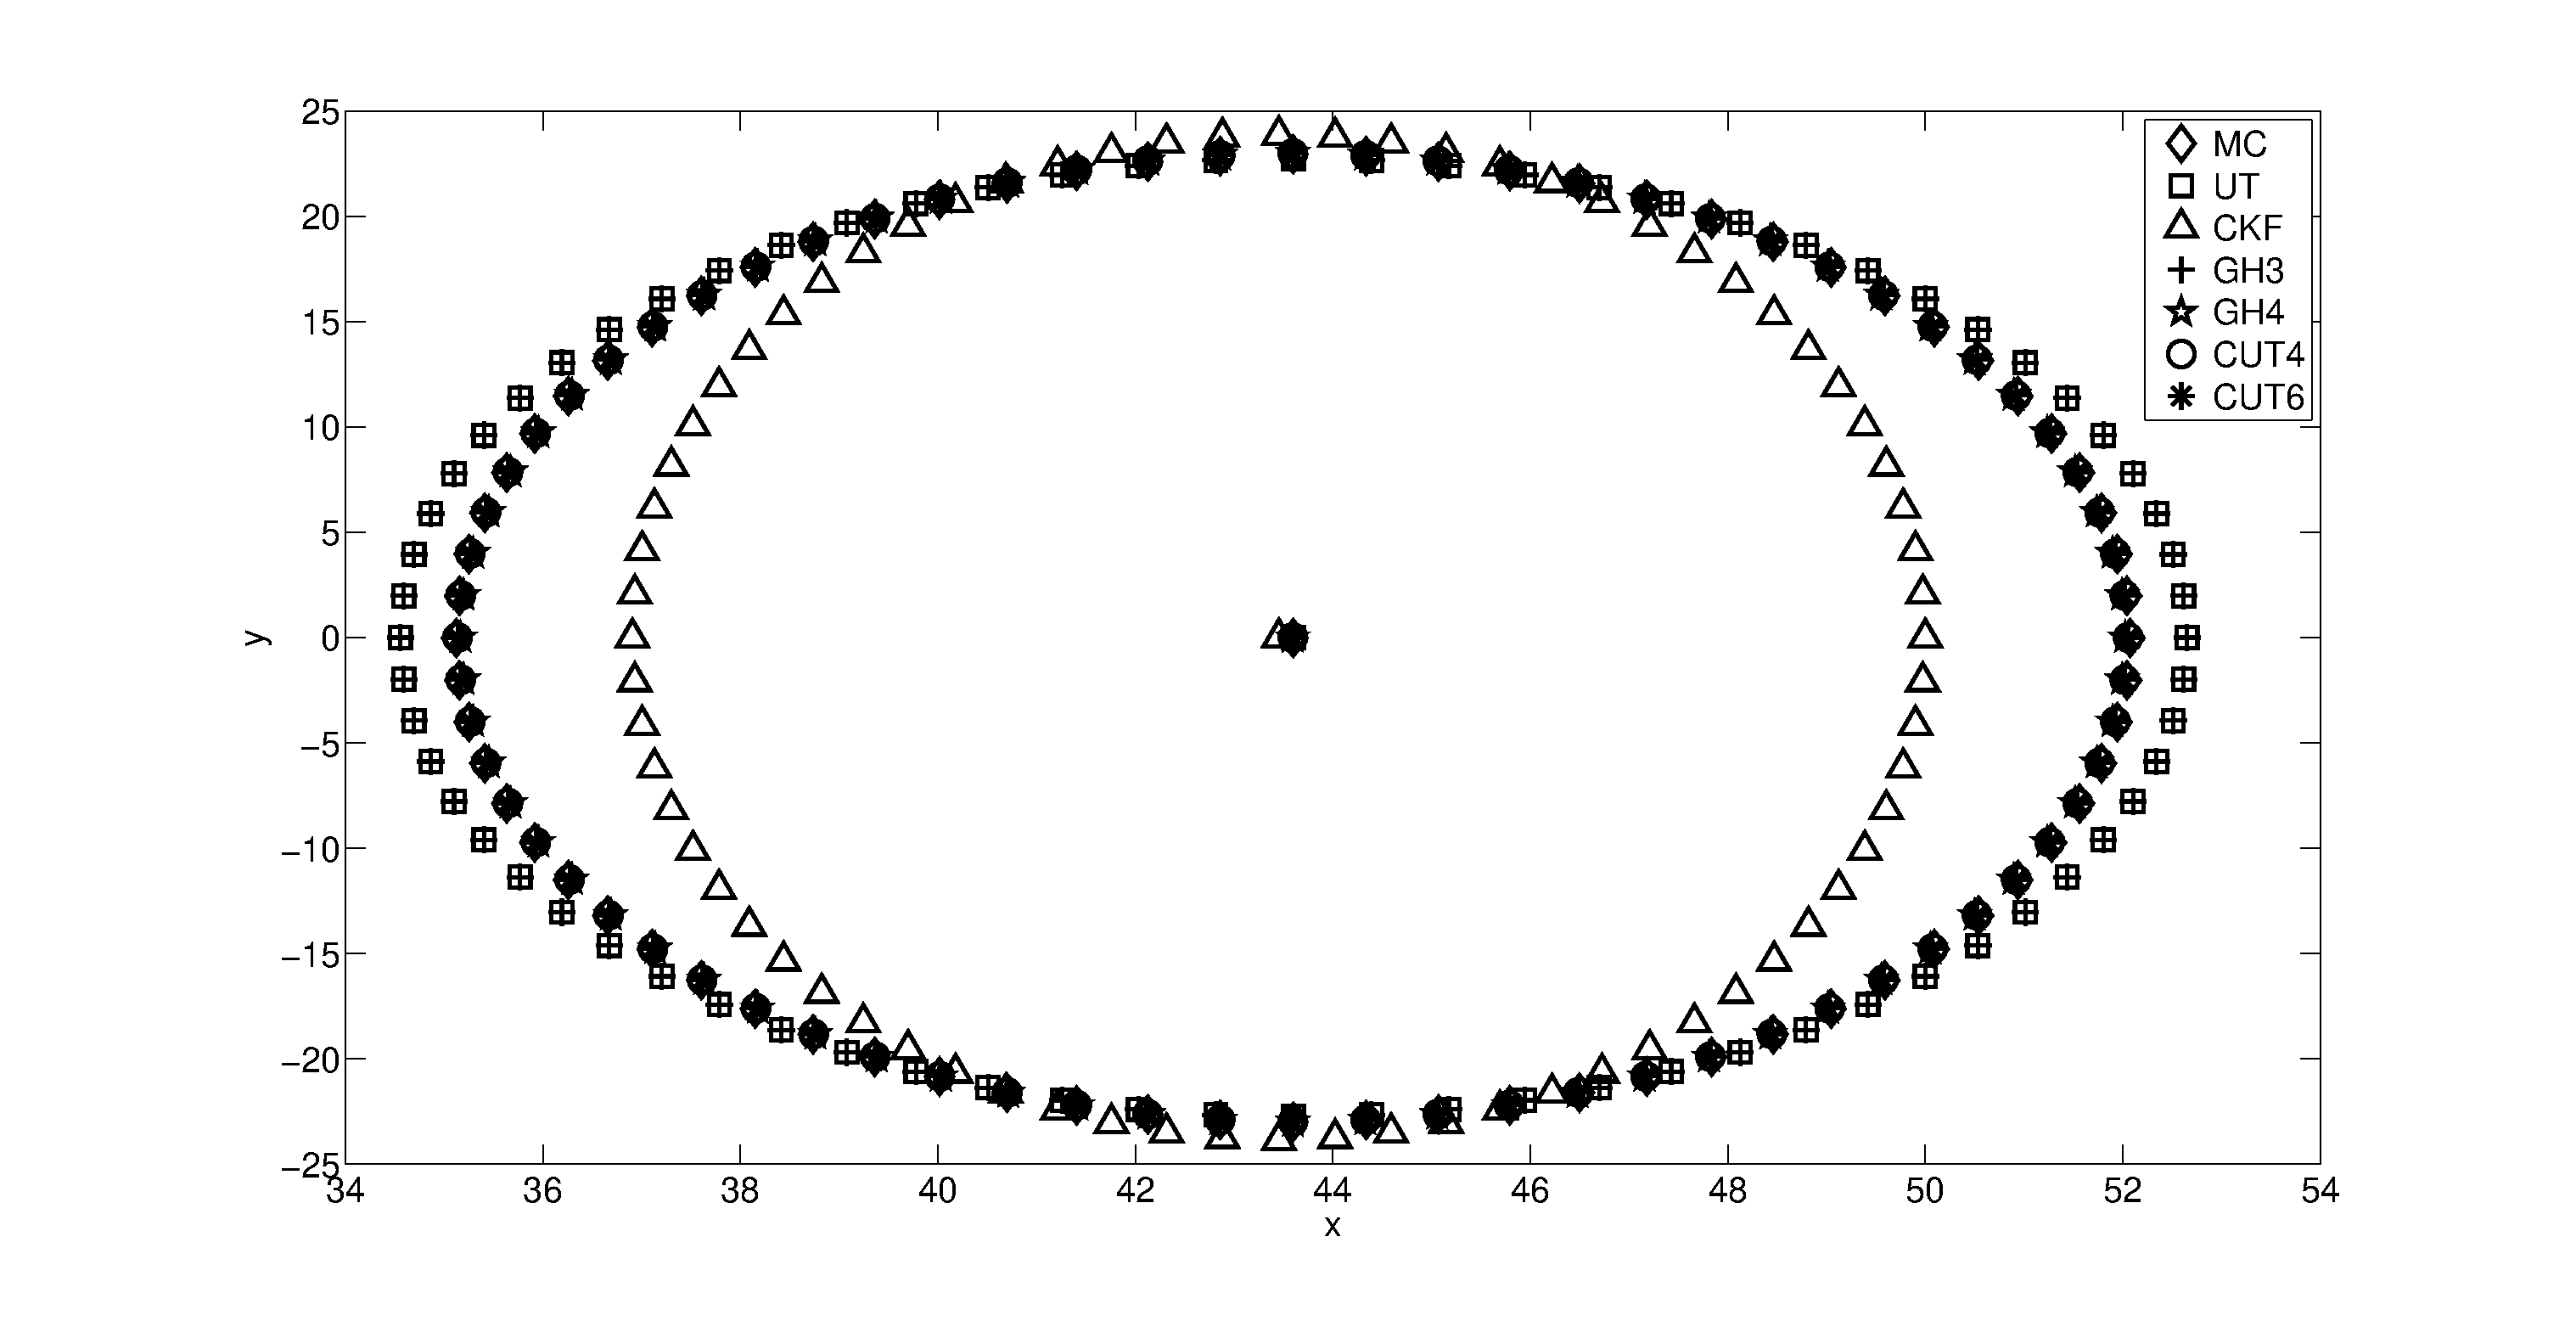
\includegraphics[width=0.5\textwidth]{polartocart3}
      \caption{2D and 3D Cubature points to satisfy 6th order moments}
      \label{fig:polartocart2}
   \end{figure}  
For the same example when the covariance for the angle is doubled, the mean for radial direction direction is 50 and the the mean for the angle is 0, the higher moment methods tend to do better as seen in Fig(\ref{fig:polartocart4})
   
   \begin{figure}[thpb]
      \centering
      \includegraphics[width=0.2\textwidth]{polar}
      \includegraphics[width=0.2\textwidth]{polartocart2}
      \caption{2D and 3D Cubature points to satisfy 6th order moments}
      \label{fig:polartocart3}
   \end{figure} 
   
   \begin{figure}[thpb]
      \centering
      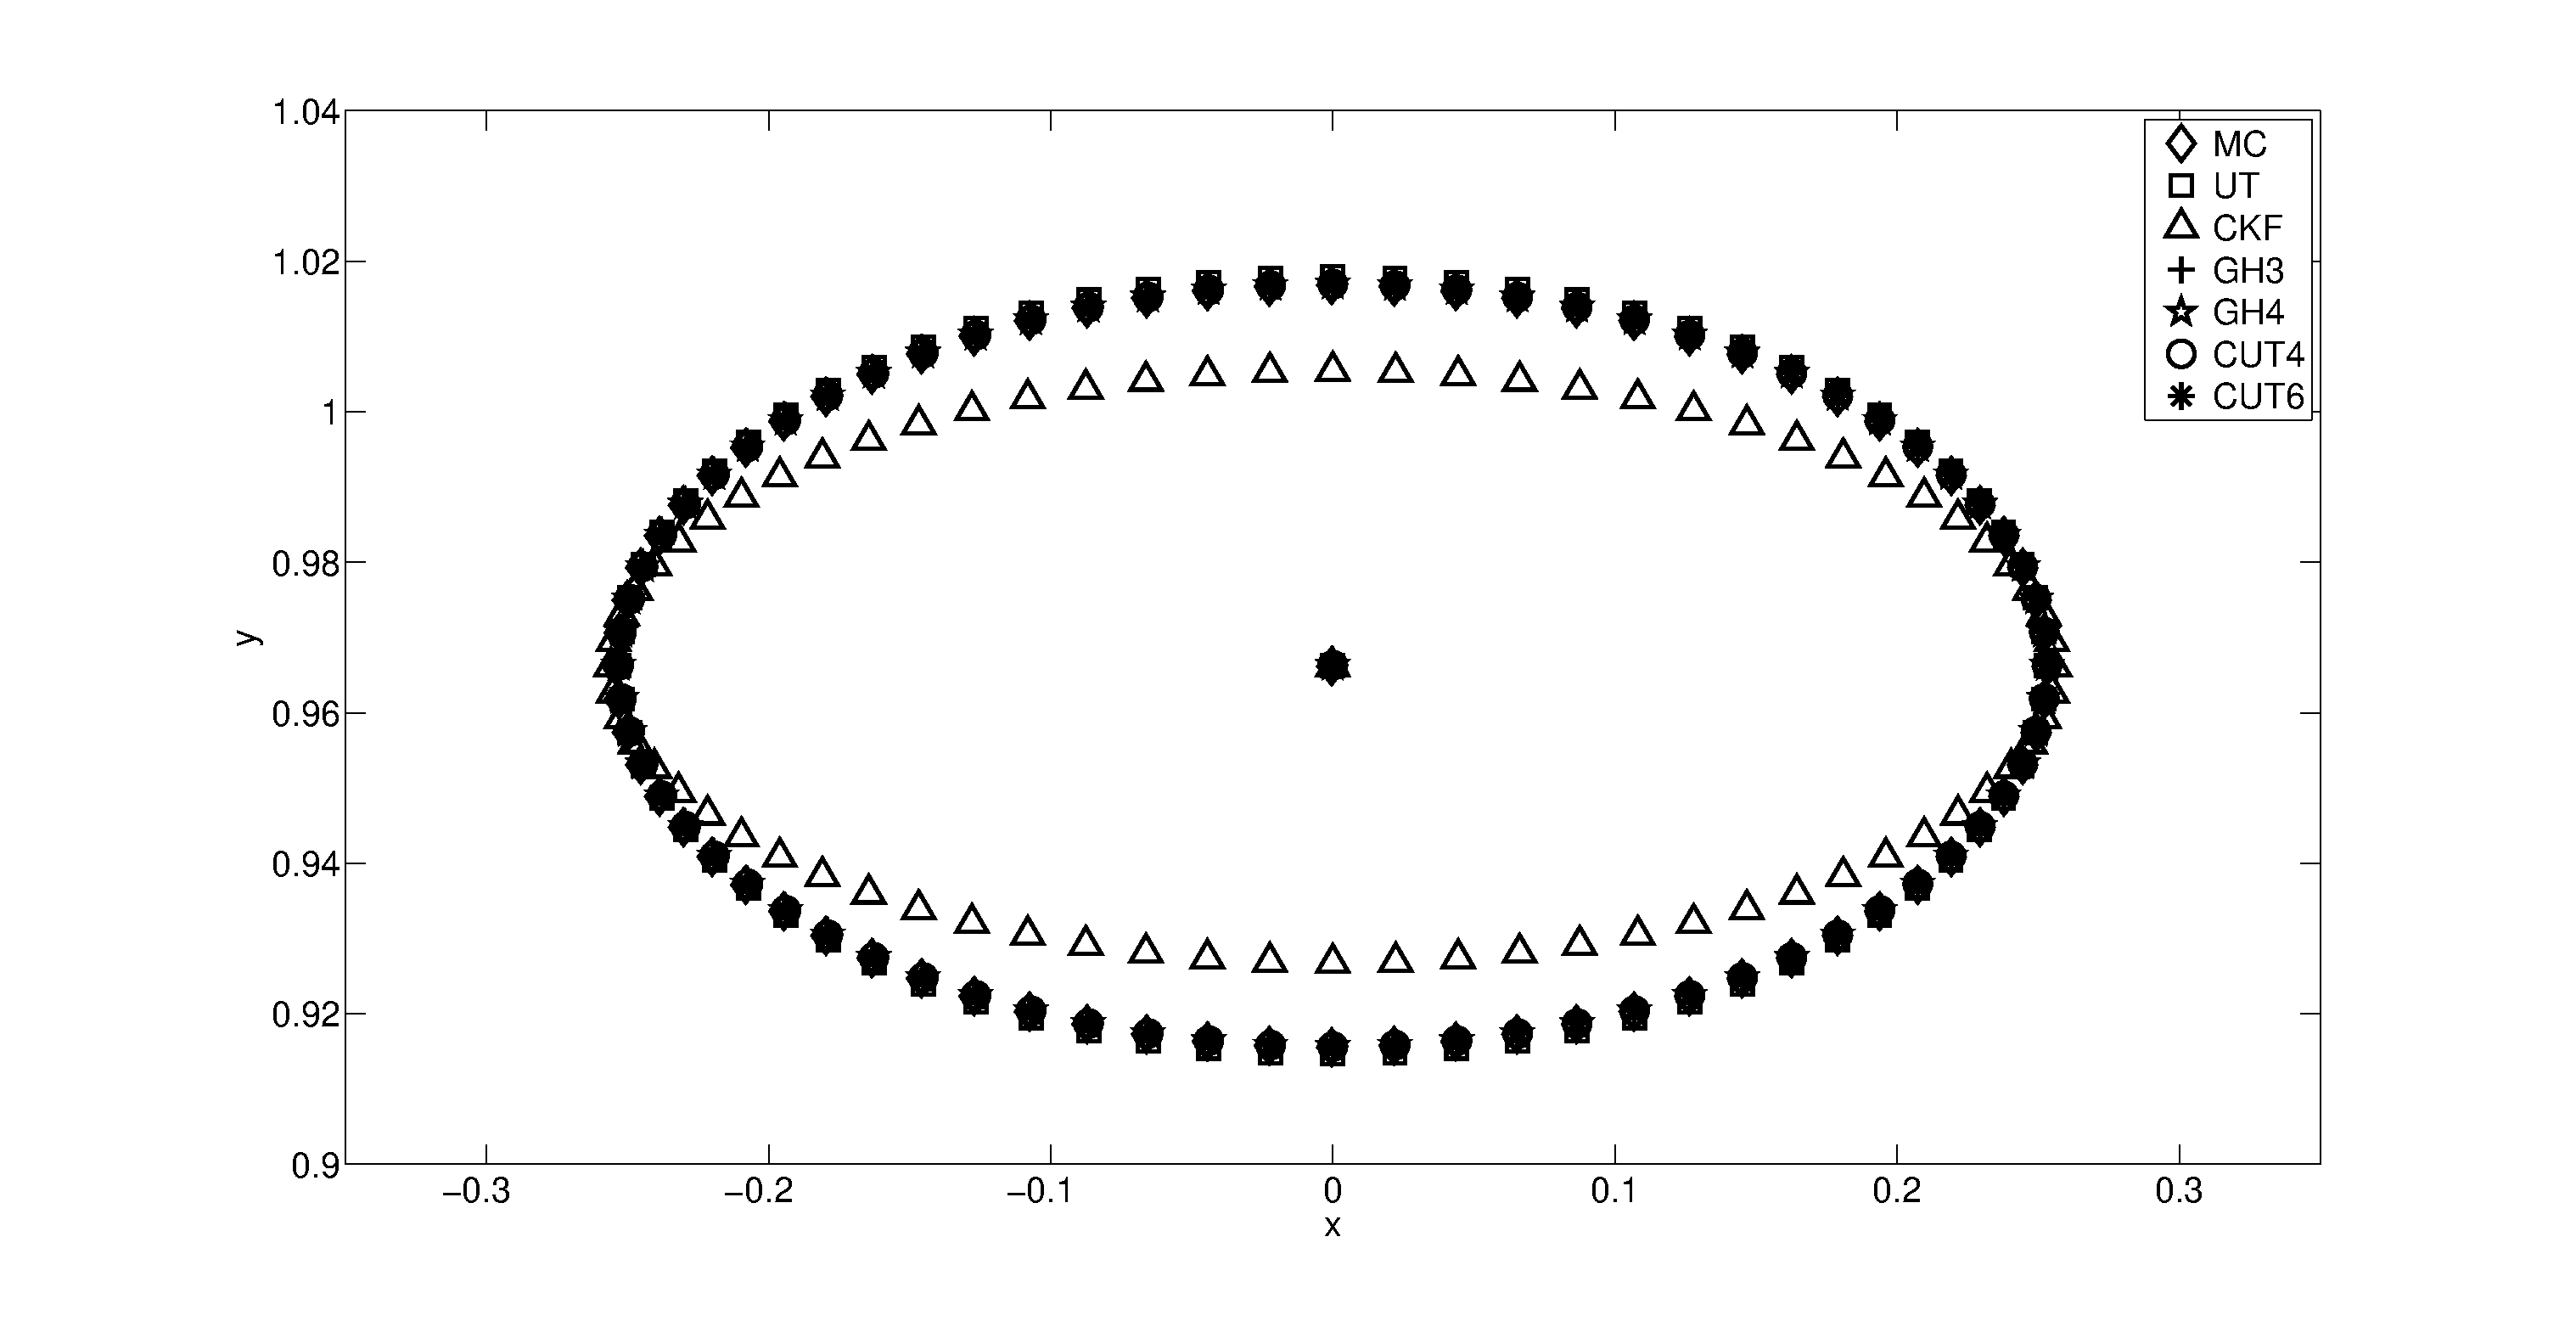
\includegraphics[width=0.5\textwidth]{polartocart}
      \caption{2D and 3D Cubature points to satisfy 6th order moments}
      \label{fig:polartocart4}
   \end{figure} 

%%%%%%%%%%%%%%%%%%%%%%%%%%
\subsubsection{$p=-3$}
Having p to be negative makes the function to behave as a delta function and hence even difficult to integrate using quadrature points. This may be because most of the quadrature points fall outside the area where the function value is near to zero and hence does not help in the integral value. The convergence of the integral is highly effected by increasing the covariance of the gaussian PDF.  This is characterised by the oscillatory type behaviour of the integral. Even taking a large number of points does not always guarantee the convergence. But by decreasing the magnitude of covariance, most of the quadrature points tend to fall within the area where the function value is significant. Under this condition one can consider the integral value to converge. This example has been shown just to motivate the fact that 'as one can capture more moments the integral value tends to converge, this statement is in agreement with equation (\ref{exptinttaylor}). The covariance is taken as $P=0.1I$ where $I$ is the identity matrix of appropriate dimension. The covariance is intentionally scaled down by $0.1$ to make the integral converge. Various methods are compared to the standard Gauss Hermite product rule.\newline
      \comments{
      \begin{figure}[thpb]
   \centering
      \includegraphics[width=0.5\textwidth]{fx_min3}
      \caption{$p=-3$ and $P=0.1I$}
      \label{fig:polartocart4}
   \end{figure} 
   }
   \begin{figure}[thpb]
   \centering
      \includegraphics[width=0.5\textwidth]{ghpmin3p01converge}
      \caption{$p=-3$ and $P=0.1I$}
      \label{fig:polartocart4}
   \end{figure} 
  \begin{figure}[thpb]
  \centering
      \includegraphics[width=0.6\textwidth]{pmin3P01}
     \includegraphics[width=0.6\textwidth]{numberofpointspmin3P01}
      \caption{$p=-3$ and $P=0.1I$}
      \label{fig:polartocart4}
   \end{figure} 
     \begin{figure}[thpb]
      \includegraphics[width=0.6\textwidth]{numberofpointspmin3P01}
      \caption{$p=-3$ and $P=0.1I$}
      \label{fig:polartocart4}
   \end{figure} 


\addtolength{\textheight}{-3cm}   % This command serves to balance the column lengths
                                  % on the last page of the document manually. It shortens
                                  % the textheight of the last page by a suitable amount.
                                  % This command does not take effect until the next page
                                  % so it should come on the page before the last. Make
                                  % sure that you do not shorten the textheight too much.

%%%%%%%%%%%%%%%%%%%%%%%%%%%%%%%%%%%%%%%%%%%%%%%%%%%%%%%%%%%%%%%%%%%%%%%%%%%%%%%%

%%%%%%%%%%%%%%%%%%%%%%%%%%%%%%%%%%%%%%%%%%%%%%%%%%%%%%%%%%%%%%%%%%%%%%%%%%%%%%%%
\section{CONCLUSIONS}
 \indent\indent Integrals involving normal weight function are extensively used in areas of statistics and nonlinear filtering....... It has been customary to use the Guass-Hermite product rule to evaluate these integrals but this not only involves a lot of computational cost but even computational time. Especially for applications in online or real-time filtering, one would prefer a cubature rule with as minimal points as possible without the compromise in accuracy. This has been a motivating factor to develop higher order sigma points. Thus we have been able to provide a sigma point set that is 4th order equivalent, a sigma point set that is 6th order equivalent till dimension 9 and finally a sigma point set that is 8th order equivalent till dimension 6. When integrating polynomial functions, each sigma point set can be considered a direct replacement for the equivalent Gauss Hermite product rule of same order.     
%%%%%%%%%%%%%%%%%%%%%%%%%%%%%%%%%%%%%%%%%%%%%%%%%%%%%%%%%%%%%%%%%%%%%%%%%%%%%%%%
\section{ACKNOWLEDGMENTS}



%%%%%%%%%%%%%%%%%%%%%%%%%%%%%%%%%%%%%%%%%%%%%%%%%%%%%%%%%%%%%%%%%%%%%%%%%%%%%%%%
\begin{thebibliography}{99}

\bibitem{c1}
Stroud A. H., Secrest D, "`Gaussian Quadrature Formulas"',Prentice hall, 1966

\bibitem{c2}
Stroud A. H., "`Approximate Calculation of Multiple Integrals"', Prentice Hall, 1971

\bibitem{c3}
Stroud A. H.,"'Numerical Integration Formulas of Degree Two"',Mathematics of Computation, Vol. 14, No. 69 (Jan., 1960), pp. 21-26

\bibitem{c4}
Philip R., Nira R.,"' Perfectly Symmetric Two-Dimensional Integration Formulas with Minimal Numbers of Points"',Mathematics of Computation, Vol. 23, No. 108 (Oct., 1969), pp. 765-779.

\bibitem{c5}
Robert Piessens and Ann Haegemans,"'Cubature Formulas of Degree Nine for Symmetric Planar Regions"',Mathematics of Computation, Vol. 29, No. 131 (Jul., 1975), pp. 810-815

\bibitem{c6}
Richard Franke,"'Minimal Point Cubatures of Precision Seven for Symmetric Planar Regions"',SIAM Journal on Numerical Analysis, Vol. 10, No. 5 (Oct., 1973), pp. 849-862

\bibitem{c7}
Michalowicz J. V., Nicholas J M,...,"'A general Isserlis theorem for mixed Gaussian random variables "', Statistics and probability letters...

\bibitem{c8}
S. J. Julier, J. K. Ulhmann and Whyte,"'A new method for nonlinear transformation of means and covariances in filters and estimators"', IEEE Trans Automat. Control vol.45, no. 3,pp 472-482 Mar. 2000

\bibitem{c9}
I Arasaratnam and Simon Haykin,"'Cubature Kalman"',IEEE transactions on Automat. Control, vol 54, no. 6, June 2009

\bibitem{c10}
SIMON J. JULIER, AND JEFFREY K. UHLMANN,"'Unscented Filtering and Nonlinear Estimation"',PROCEEDINGS OF THE IEEE, VOL. 92, NO. 3, MARCH 2004

\bibitem{c11}
A. H. Stroud,"'Some Fifth Degree Integration Formulas for Symmetric Regions"',Mathematics of Computation, Vol. 20, No. 93 (Jan., 1966), pp. 90-97

\bibitem{c12}
A. H. Stroud,"'Some Seventh Degree Integration Formulas for Symmetric Regions"',SIAM Journal on Numerical Analysis, Vol. 4, No. 1 (Mar., 1967), pp. 37-44


\end{thebibliography}

\end{document}
